\ctitle{Simulation}
We are concerned with solving the IVP
\begin{equation}
    \Dot{y} = f(y,t), \quad y(t_0) = y_0
\end{equation}
The Jacobian of the system is defined as
\begin{equation}
    J = \frac{\partial f}{\partial y}(y,t)
\end{equation}
Note that the Jacobian is $A$ for a linear, time-invariant system $\dot{x} = Ax + Bu$.

\section{Explicit Runge-Kutta methods}

An explicit Runge-Kutta method with $σ$ stages for the system
\begin{equation}
    \dot{\mathbf{y}}=\mathbf{f}(\mathbf{y}, t)
\end{equation}

is given by

\begin{equation}
    \mathbf{k}_{i}=\mathbf{f}\left(\mathbf{y}_{n}+h \sum_{j=1}^{i-1} a_{i j} \mathbf{k}_{j}, t_{n}+c_{i} h\right), i=1, \ldots, \sigma
\end{equation}

\begin{equation}
\mathbf{y}_{n+1}=\mathbf{y}_{n}+h \sum_{j=1}^{\sigma} b_{j} \mathbf{k}_{j}
\end{equation}

The explicit Runge-Kutta method can be written out as
\begin{equation}
    \begin{aligned}
        \mathbf{k}_{1}=& \mathbf{f}\left(\mathbf{y}_{n}, t_{n}\right) \\
        \mathbf{k}_{2}=& \mathbf{f}\left(\mathbf{y}_{n}+h a_{21} \mathbf{k}_{1}, t_{n}+c_{2} h\right) \\
        \mathbf{k}_{3}=& \mathbf{f}\left(\mathbf{y}_{n}+h\left(a_{31} \mathbf{k}_{1}+a_{32} \mathbf{k}_{2}\right), t_{n}+c_{3} h\right) \\
        & \vdots \\
        \mathbf{k}_{\sigma}=& \mathbf{f}\left(\mathbf{y}_{n}+h\left(a_{\sigma 1} \mathbf{k}_{1}+\ldots+a_{\sigma, \sigma-1} \mathbf{k}_{\sigma-1}\right), t_{n}+c_{\sigma} h\right) \\
        \mathbf{y}_{n+1}=& \mathbf{y}_{n}+h\left(b_{1} \mathbf{k}_{1}+\ldots+b_{\sigma} \mathbf{k}_{\sigma}\right)
    \end{aligned}
\end{equation}

Each explicit Runge-Kutta method is described by its parameters, $a_{ij}$ , $b_i$ and $c_i$, which can be arranged in a \textit{Butcher array} of the form

\begin{figure}[H]
    \centering
    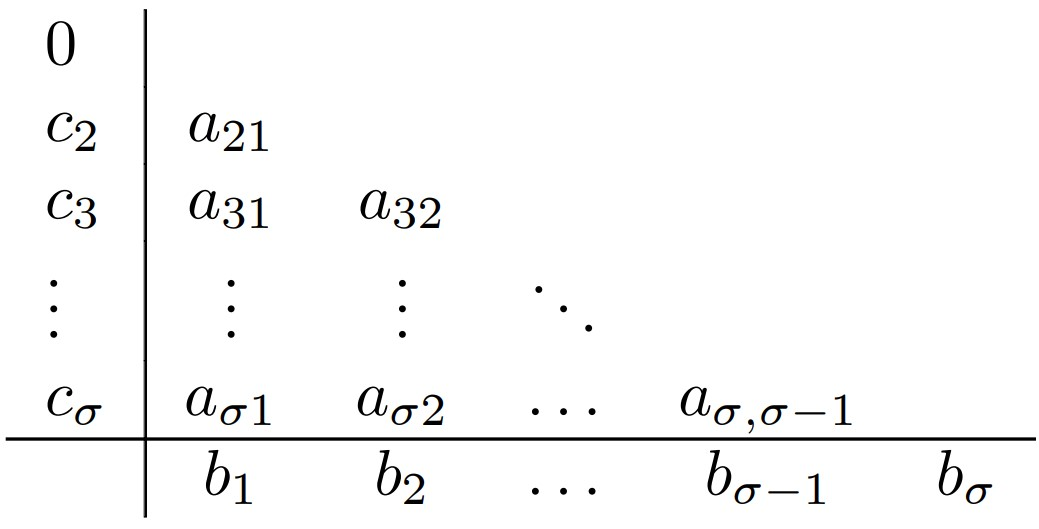
\includegraphics[width=0.5\textwidth]{images/butcher.jpg}
    \label{fig:butcher}
\end{figure}

If all non-zero entires of the matrix A are below the diagonal, then the method is \underline{explicit}. Otherwise, the method is \underline{implicit}.

\textbf{Example}: The 4th-order Runge-Kutta method

\begin{equation}
    \begin{aligned}
        k_{1} &=f\left(t_{n}, y_{n}\right) \\
        k_{2} &=f\left(t_{n}+\frac{h}{2}, y_{n}+\frac{h}{2} k_{1}\right) \\
        k_{3} &=f\left(t_{n}+\frac{h}{2}, y_{n}+\frac{h}{2} k_{2}\right) \\
        k_{4} &=f\left(t_{n}+h, y_{n}+h k_{3}\right) \\
        y_{n+1} &=y_{n}+\frac{h}{6}\left(k_{1}+2 k_{2}+2 k_{3}+k_{4}\right)
    \end{aligned}
\end{equation}

is equivalent to

\begin{equation}
    \begin{array}{c|cccc}
    0 & & & & \\
    \frac{1}{2} & \frac{1}{2} & & & \\
    \frac{1}{2} & 0 & \frac{1}{2} & & \\
    1 & 0 & 0 & 1 & \\
    \hline & \frac{1}{6} & \frac{1}{3} & \frac{1}{3} & \frac{1}{6}
    \end{array}
\end{equation}

\vspace{0.25cm}

\textbf{Example}: Task 3 (15th May, Exam 2019)

\begin{equation}
\begin{array}{c|cc}
\gamma & \gamma & 0 \\
1-\gamma & 1-2 \gamma & \gamma \\
\hline & 1 / 2 & 1 / 2
\end{array}
\end{equation}

is equivalent to

\begin{equation}
    \begin{aligned}
        \mathbf{k}_{1} &=\mathbf{f}\left(\mathbf{y}_{n}+\gamma h \mathbf{k}_{1}, t_{n}+\gamma h\right), \\
        \mathbf{k}_{2} &=\mathbf{f}\left(\mathbf{y}_{n}+(1-2 \gamma) h \mathbf{k}_{1}+\gamma h \mathbf{k}_{2}, t_{n}+(1-\gamma) h\right), \\
        \mathbf{y}_{n+1} &=\mathbf{y}_{n}+\frac{1}{2} h \mathbf{k}_{1}+\frac{1}{2} h \mathbf{k}_{2}
    \end{aligned}
\end{equation}

\textbf{Example}: Task 1 (June, Exam 2016) \\
Showing an implicit Runge-Kutta with three stages. (Implicit as non-zero elements on the diagonal of the A-matrix implies that the method is implicit
\begin{equation}
    \begin{aligned}
        \mathbf{k}_{1} &=\mathbf{f}\left(\mathbf{y}_{n}, t_{n}\right) \\
        \mathbf{k}_{2} &=\mathbf{f}\left(\mathbf{y}_{n}+\frac{h}{4} \mathbf{k}_{1}+\frac{h}{4} \mathbf{k}_{2}, t_{n}+\frac{h}{2}\right) \\
        \mathbf{k}_{3} &=\mathbf{f}\left(\mathbf{y}_{n}+h \mathbf{k}_{2}, t_{n}+h\right) \\
        \mathbf{y}_{n+1} &=\mathbf{y}_{n}+\frac{h}{6}\left(\mathbf{k}_{1}+4 \mathbf{k}_{2}+\mathbf{k}_{3}\right)
    \end{aligned}
\end{equation}

is equivalent to \\

\begin{equation}
    \begin{array}{c|ccc}
        0 & & & \\
        1 / 2 & 1 / 4 & 1 / 4 & \\
        1 & 0 & 1 & \\
        \hline & 1 / 6 & 2 / 3 & 1 / 6
    \end{array}
\end{equation}

\section{Stability functions}
The stability of a numerical method is ensured if $|R(h\lambda_i)| \leq 1$ for all eigenvalues $\lambda_i$.\\
Higher order stability function : $R(h \lambda)=1+\lambda h+\frac{1}{2} \lambda^{2} h^{2}$\\
\subsection{ERK methods}
\begin{equation}
    R_E(h\lambda) = \det \left[ I - h\lambda (A - \mathbf{1} b^\top) \right], \enskip \text{where} \enskip  \mathbf{1} = (1, ... , 1)^\top
\end{equation}
Note that $R_E(h\lambda)$ will be a polynomial in $h\lambda$ of order less than or equal to $\sigma$ (the number of stages).

\subsection{IRK methods}
\begin{align}
    R(h\lambda) = \left[ 1 + h\lambda b^\top (I-h\lambda A)^{-1} \mathbf{1} \right]\\
    R(h\lambda) = \frac{\det \left[ I - h\lambda(A - \mathbf{1}b^\top) \right]}{\det(I - h\lambda A)}
\end{align}

\section{Stability of RK methods}

\subsection{Aliasing}
The \textit{Nyquist frequency} is half of the sampling rate
\begin{equation}
    \omega_{\text{Nyquist}} = \frac{1}{2} \cdot \frac{2\pi}{h}, \enskip \text{where $h$ is the step size.}
\end{equation}
Two systems oscillating at a low frequency $\omega < \omega_{\text{Nyquist}}$ and a high frequency $\omega + 2k\frac{\pi}{h} > \omega_{\text{Nyquist}}$ ($k$ integer) will intercept at all sampling points, and therefore a solver will not be able to distinguish them. More specifically, the solver will believe that the system with higher frequency is the system with lower frequency, when fitting the curve.

\subsection{A- and L-stability}
\textbf{Definition:} A method is A-stable if \\ $|R(h\lambda)| \leq 1 \enskip \forall \enskip \operatorname{Re} \lambda \leq 0$.\\
This definitions means that an A-stable method is stable for all stable test systems $\dot{y} = \lambda y$. Note also that no ERK method can be A-stable, since $|R_E(h\lambda)| \to \infty$ as $|\lambda| \to \infty$.\\
\textbf{Definition:} A method is L-stable if it is A-stable and $|R(j\omega h)| \to 0$ when $\omega \to \infty \enskip \forall$ systems $\dot{y} = j\omega y$.\\
A-stable methods can suffer from aliasing for systems with fast dynamics (faster than Nyquist frequency), whereas an L-stable method will simply damp out these fast dynamics. This means that the L-stable method might give a better qualitative representation of what the actual solution looks like.

\subsection{Stiffly accurate methods and algebraic stability}
\textbf{Definition:} A method is stiffly accurate if
\begin{equation}
    \det(A) \neq 0 \text{ and } b = A^\top [0, 0, ..., 1]^\top
\end{equation}
Note: A-stable and stiffly accurate $\implies$ L-stable.\\
\textbf{Definition:} A method is algebraically stable if 
\begin{equation} 
    M = \operatorname{diag}(b)A + (\operatorname{diag}(b)A)^\top + bb^\top
\end{equation}
is positive semi-definite. Note: Algebraically stable $\implies$ A-stable.

\section{DAEs}
Used a lot in the modelling of complex and large-scale systems. DAEs are a set of equations that do not directly define the entire state. Has many forms, but usually: if the implicit ODE $F(\dot{x}, x, u, t)=0$ and it's $det(\frac{\partial F}{\partial \dot{x}}) = 0$ then its a DAE. Method for finding index (one way to go about it):
\begin{itemize}
    \item Differentiate algebraic equation(s) $g(x, z, u)$ until you can solve for the algebraic variable(s).
    \item The DAE system is now index 1. If you differentiated $p$ times in the previous step, the index is $p+1$.
\end{itemize}
\textbf{Differential index}, number of times we need to differentiate to transform DAE to ODE.\\
\textbf{Index reduction}, is the differentiate the DAE to be one differentiation from ODE.
\begin{figure}[H]
    \centering
    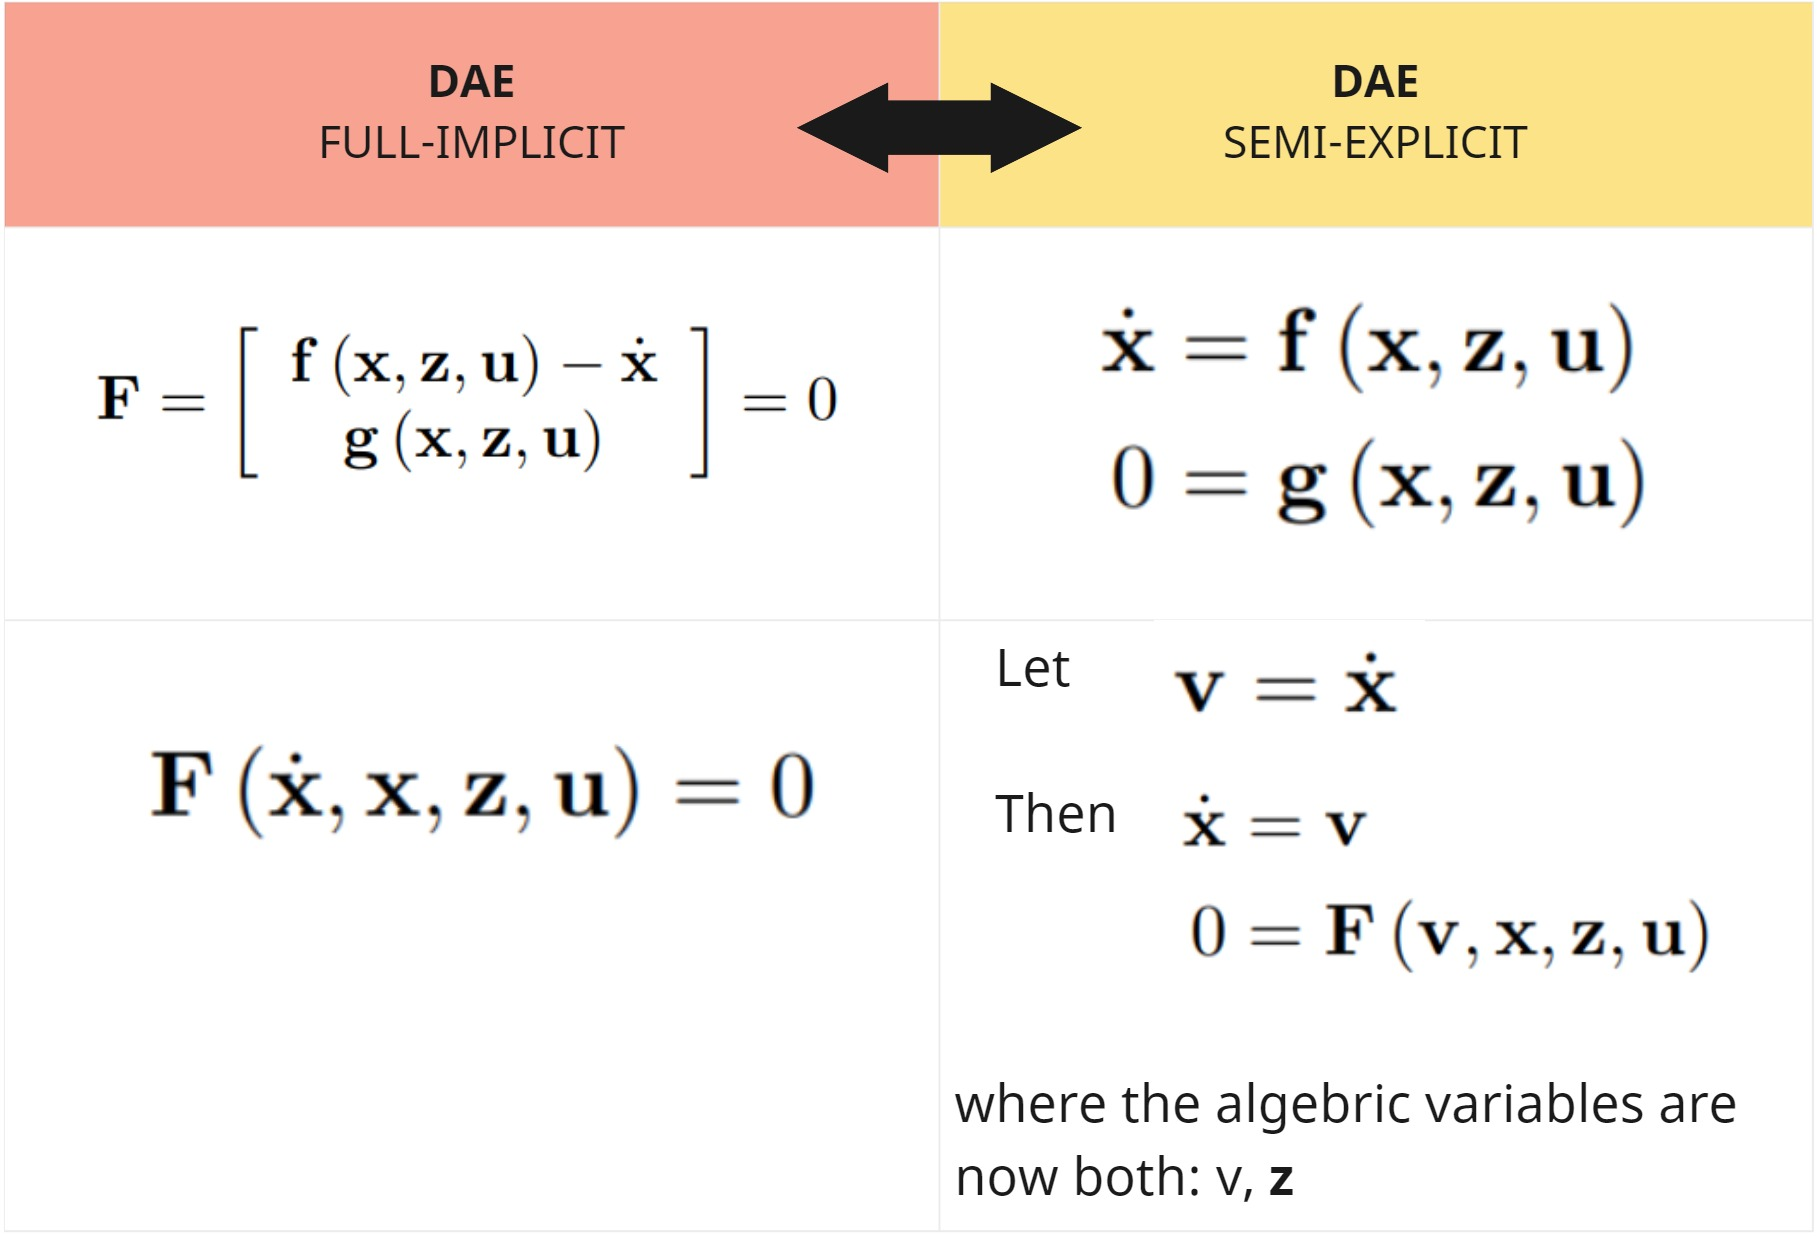
\includegraphics[width=0.5\textwidth]{images/dae_full_vs_semi.jpg}
    \label{fig:dae_exp}
\end{figure}

\textbf{Example}: Finding differential index \\
Given eq. \ref{eq:semi_example}

\begin{equation} \label{eq:semi_example}
    \begin{aligned}
        &\dot{\mathrm{x}}=\mathrm{f}(\mathrm{x}, \mathrm{z}, \mathrm{u}) \\
        &0=g(\mathrm{x}, \mathrm{z}, \mathrm{u})
    \end{aligned}
\end{equation}

if a single time differentiation on the algebraic equation \textit{g}, yields an ODE - then this means eq. \ref{eq:semi_example} is an Index-1 DAE.
\hfill \break

\textbf{Example}: Fully-Implicit to Semi-Explicit \\
Given eq. \ref{eq:full_exp}
\begin{equation}\label{eq:full_exp}
    \begin{aligned}
        m \ddot{x} &=-2 x \mu \\
        m \ddot{y} &=-m g-2 y \mu \\
        l^{2} &=x^{2}+y^{2}
    \end{aligned}
\end{equation}
let $q=(x, y)^{T}, v=\left(x^{\prime}, y^{\prime}\right)^{T}$, then 

\begin{equation}
    \begin{aligned}
        q^{\prime} &=v \\
        v^{\prime} &=\frac{1}{m}\left(-2 \mu q+\left(\begin{array}{c}
        0 \\
        -m g
        \end{array}\right)\right) \\
        0 &=x^{2}+y^{2}-l^{2}=q^{T} q-l^{2}
        \end{aligned}
\end{equation}

\subsubsection{Simulation}
To simulate them, we need consistency conditions for it to be well-defined. We need to reduce it twice (differentiate the constrains twice, e.g. DAE Idx 3 => DAE Idx 1). If we reduce the constraints, we get “hidden constraints”. $\dot{c}(q(0)) = 0$ (might have linear drift), $\ddot{c}(q(0)) = 0$.

We might also get constraint drift. Can be reduced using “Baumgarte” stabilization.
\begin{equation}
    \ddot{c} + 2\alpha\dot{c} + \alpha^2c > 0
\end{equation}
(we substitute the $\ddot{c}(q(0))$ constraint)


\section{Advanced topics}

\subsection{Automatic adjustment of step size}
The step size $h$ can be selected so that the desired accuracy is obtained. Variable-step methods are useful for stiff systems (large spread in eigenvalues of Jacobian) and systems with strong nonlinearities (eigenvalues of Jacobian of linearization change a lot for each time step).

Idea: Estimate local error and adjust $h$ such that the local error is less than the specified tolerance.

Implementation:
\begin{enumerate}
    \item Compute the next iteration with two different methods: $y_{n+1}$ with a method of order $p$ and ${\hat{y}_{n+1}}$ with a method of order $\hat{p} = p+1$.
    \item The local exact solution is then
    \begin{equation}
        y_L(t_n;t_{n+1}) = y_{n+1} + e_{n+1} = \hat{y}_{n} + \hat{e}_{n+1}
    \end{equation}
    with $e_{n+1} = O(h^{p+1})$ and $\hat{e}_{n+1} = O(h^{p+2})$.
    \item Since $\hat{e}_{n+1} \ll e_{n+1}$, we get the following 
    \begin{equation}
        y_{n+1} - \hat{y}_{n} = e_{n+1} - \hat{e}_{n+1} \approx e_{n+1}
    \end{equation}
    $h$ can then be chosen such that the local error $e_{n+1}$ is as small as desired.
\end{enumerate}

Since $\hat{y}_{n+1}$ is computed with a higher-order method than $y_{n+1}$, it would make sense to use that for the next iteration instead, this is called local extrapolation. Whichever solution is chosen as $\hat{y}_{n+1}$ is called the \emph{embedded solution}.

\subsection{Event detection}
Let the event be given by
\begin{equation}
    g(y,t) = 0
\end{equation}
e.g. a bouncing ball hitting the floor (crossing the $x$-axis). By checking for sign changes in $g$ for each iteration, the time $t_n + \alpha$ of the event can be found by solving
\begin{equation}
    g[y_n(\alpha), t_n + \alpha h] = 0
\end{equation}
for $\alpha \in [0,1]$, where $y_n(\alpha)$ is the \emph{dense output} found with interpolation (see page 565).

\subsection{Multistep methods}
A one-step method only uses the previous value $y_n$ to compute $y_{n+1}$. A multistep method, on the other hand, uses $y_{n-1}$, $y_{n-2}$, etc. as well. The scheme looks like this:
\begin{equation}
    \begin{split}
    y_{n+1} &= \alpha_1 y_n + \alpha_2 y_{n-1} + \dots \\ &+ h(\beta_0 f(y_{n+1}, t_{n+1}) + \beta_1 f(y_n, t_n) + \beta_2 f(y_{n-1}, t_{n-1}) + \dots)
    \end{split}
\end{equation}
The parameters/weights are derived by curve fitting polynomials to the previous time steps.
The known stability concepts from one-step methods apply to multistep methods as well.